\subsection {Session 10, Exercise 6}

\lineparagraph {Exercise}

Some rungs of a ladder of $f$ rungs are so rotten that if someone steps on them, then they break. Fortunately, it known which rungs are so bad. We can step over three rungs at most in one step. Give a dynamic programming algorithm that determines

\begin{enumerate}[a)]
    \item whether we can climb up on the top of the ladder from the bottom,
    \item how many ways can we reach the top rung?
\end{enumerate}

(It is assumed that one can step on the top rung.) What is the running time of your algorithm?

\lineparagraph {Solution}

\begin{itemize}
    \item The exercise is asking if we can reach the $f$th step. To reach the $f$th step we could come from the $(f-1)$, $(f-2)$, $(f-3)$ or $(f-4)$th steps, since we can step over $3$ steps.
\end{itemize}

\begin{center}
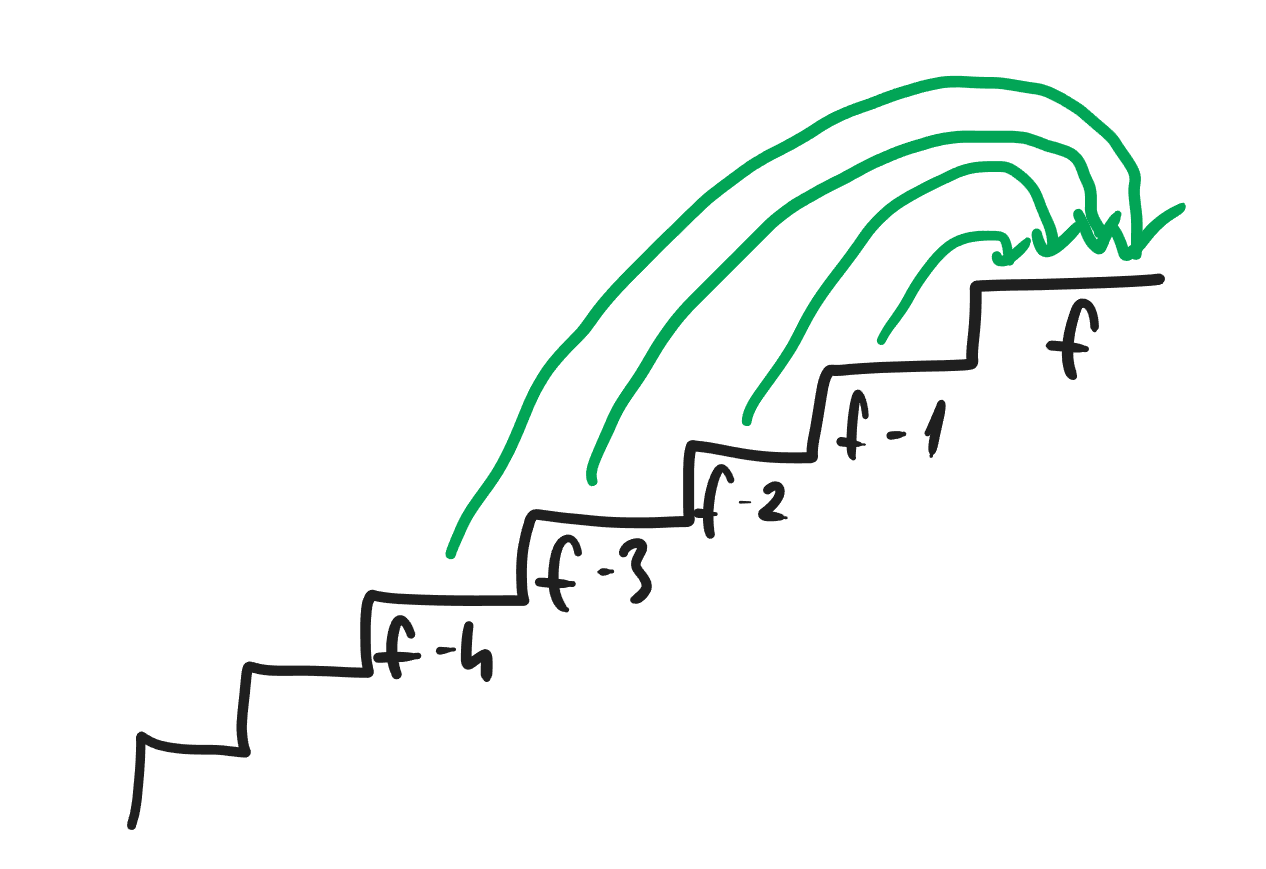
\includegraphics[width=0.7\linewidth]{10/06/ladder_steps.png}
\end{center}

\begin{itemize}
    \item Side note: I would argue that stepping over 3 steps looks like this:
\end{itemize}

\begin{center}
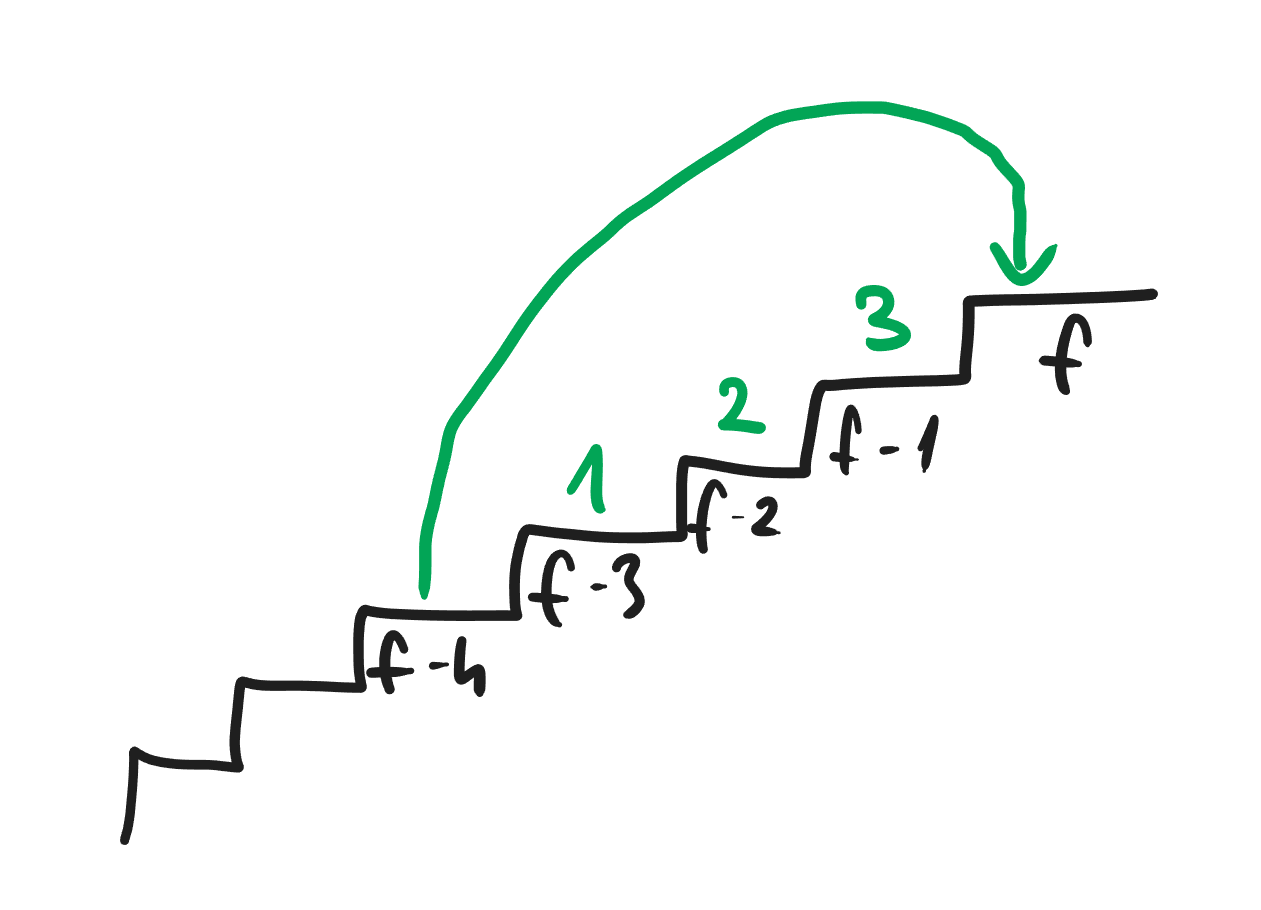
\includegraphics[width=0.7\linewidth]{10/06/ladder_step_over_3.png}
\end{center}

\begin{itemize}
    \item But many of you have argued that it looks like this instead:
\end{itemize}

\begin{center}
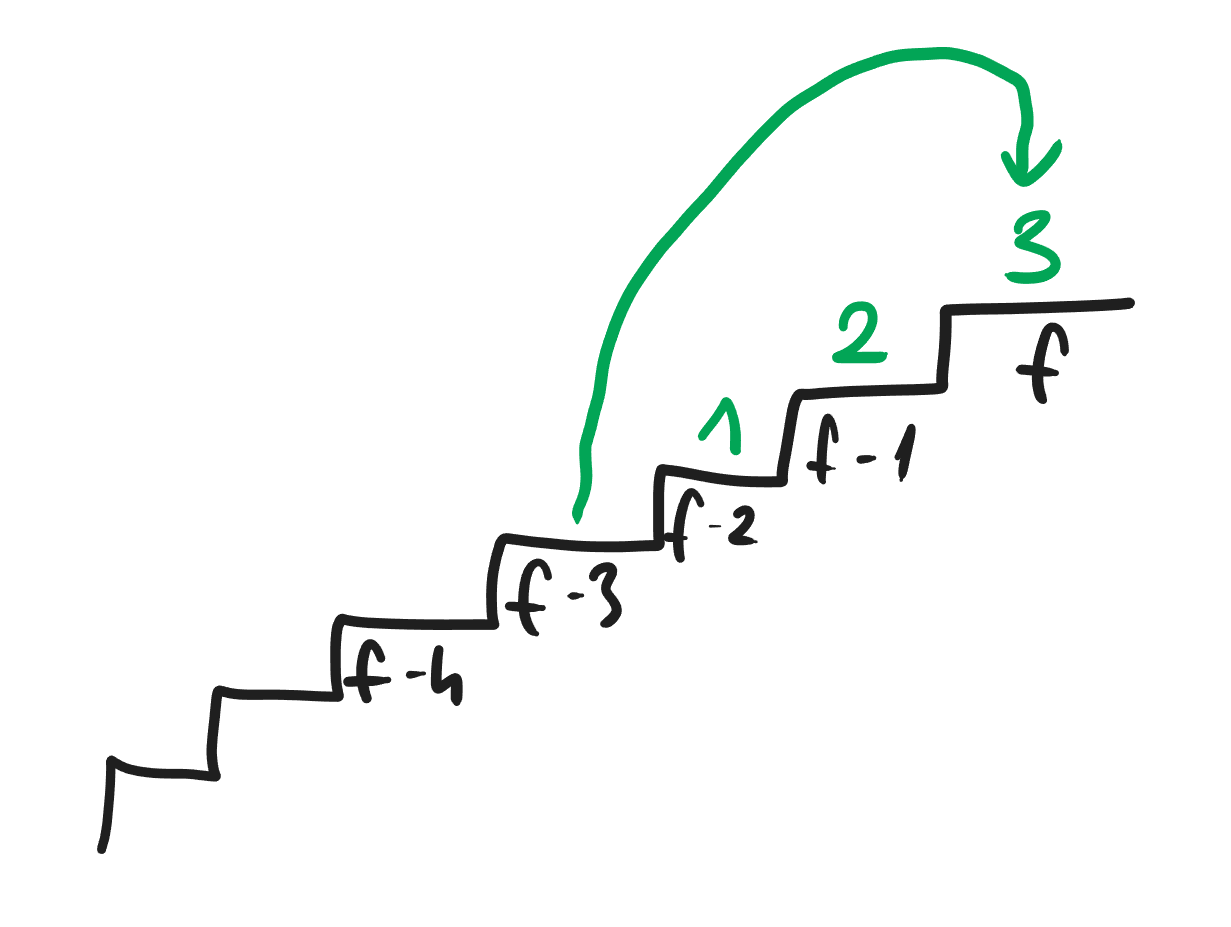
\includegraphics[width=0.7\linewidth]{10/06/ladder_steps_other.png}
\end{center}

\begin{itemize}
    \item I think it depends on how you interpret the word 'over', if you interpret it to mean 'stepping above the steps without touching them', then it means the first drawing, while if you interpret it as 'stepping forwards/upwards that many steps', then it means the second drawing. In either case, it doesn't really matter here and if you're not sure during the exam, always ask the instructors present for clarification.
\end{itemize}

Back to the exercise:

\begin{itemize}
    \item The exercise is asking if we can reach the $f$th step. To reach the $f$th step we could come from the $(f-1)$, $(f-2)$, $(f-3)$ or $(f-4)$th steps. This is our \textbf{key statement}.
    \item If we store if we can reach the $i$th step from the bottom (let's say that's the 0th step) in a 1D array $A$ indexed from $0$ to $f$ ($\rightarrow$ \textbf{Step 1}: Define $A$, what $A[i]$ means?), then $A[f] = A[f-1] \lor{} A[f-2] \lor{} A[f-3] \lor{} A[f-4]$, where $\lor{}$ is the logical or symbol.
    \item Or, in general for any $i$th step: $A[i] = A[i-1] \lor{} A[i-2] \lor{} A[i-3] \lor{} A[i-4]$.
    \item And to deal with broken steps, let's say that $B[i]$ is $True$ if the $i$th step is steppable and $False$ if not. Now we can say that $A[i]$ must be steppable \textbf{and} we must be able to step on any of the previous steps:
    \item $A[i] = B[i]\land{}(A[i-1] \lor{} A[i-2] \lor{} A[i-3] \lor{} A[i-4])$ ($\rightarrow$ \textbf{Step 2}: Generic recursive formula.), where $\land{}$ is the logical and symbol.
    \item The base case is $A[0] = True$, since we are standing on the floor at the bottom.
    \item This recursive formula breaks down the moment $i<4$, we will start to index $A$ with negative numbers, whenever we indexed with a negative number we should remove that $A[i]$ from the or.
    \item Let's just say that $A[i] = False$, for $i<0$, because I'm lazy and $A[0] = True$. ($\rightarrow$ \textbf{Step 3}: Base cases.)
    \item We can fill out the $A$ from index $0$ to $f$, so the solutions for the previous indexes are already available for us when calculating the current value. ($\rightarrow$ \textbf{Step 4}: Order in which $A$ is filled.)
    \item The solution is in $A[f]$, it is $True$ if we can reach the $f$th step and $False$ if not. ($\rightarrow$ \textbf{Step 5}: Where is the solution?)
    \item The runtime complexity: we fill out an array of size $f+1$, and in each step we reach back to $4$ other values plus a value in $B$ and do some logical operators between them. So each step can be done in constant time, so the runtime complexity is $O(n)$ in total. ($\rightarrow$ \textbf{Step 6}: Runtime complexity.)
\end{itemize}

And the second task:

\begin{itemize}
    \item The backbone of the algorithm is going to be the same, we only need to slightly tweak our  calculations: switch from boolean logic to integers.
    \item Usually to go from boolean logic to integers: switch and to multiplication, switch or to addition, and switch $False$ to $0$ and $True$ to $1$.
    \item So change this:
\end{itemize}

\begin{align*}
A[i] = B[i]\land{}(A[i-1] \lor{} A[i-2] \lor{} A[i-3] \lor{} A[i-4])
\end{align*}

\begin{itemize}
    \item Into this:
\end{itemize}

\begin{align*}
A[i] = B[i]\cdot{}(A[i-1] + A[i-2] + A[i-3] + A[i-4])
\end{align*}

\begin{itemize}
    \item So now $B[i]$ should be $1$ if the $i$th step is steppable and $0$ if not, so there will be $0$ ways to reach unsteppable steps as intended.
    \item And $A[i]$ will contain how many ways the $i$th step is reachable.
    \item $A[i] = 0$ for $i<0$ and $A[0] = 1$.
    \item The rest is the same.
\end{itemize}